%%%%%%%%%%%%%%%%%%%%%%%%%%%%%%%%%%%
%%%%%%%%% Modeling Chapter %%%%%%%%
%%%%%%%%%%%%%%%%%%%%%%%%%%%%%%%%%%%
\label{ch: modeling}

%%% Section overview





%%%%%%%%%%%%%%%%%%%%%%%%%%%%%%%%%%%
%%%% Analytic Impedance Model %%%%%
%%%%%%%%%%%%%%%%%%%%%%%%%%%%%%%%%%%
\section{Analytic Single Cell Impedance Model}
\par For cell suspensions with low volume fractions, Maxwell's Mixture theory can model the electrical impedance of the system. The model is summarized in equations \ref{} to \ref{}. For a full description, see section \ref{sec:maxwell_mixture_theory} and \ref{sec:electrode_cell_constant}.

\begin{equation}
    \Tilde{Z}_{mix} = \frac{1}{jw\Tilde{C}}
\end{equation}
\begin{equation}
    \Tilde{C} = \Tilde{\epsilon}_{mix}G_f    
\end{equation}
\begin{equation}
    \Tilde{\epsilon}_{mix} = \Tilde{\epsilon}_m \frac{1 + 2\phi\Tilde{f}_{cm}}{1-\phi\Tilde{f}_{cm}}
\end{equation}
\begin{equation}
\end{equation}

\par The $d$ and $\gamma$ in equation ?? refer to the distance between and the height of the two electrodes in the ideal plate capacitor model in figure ??. To find $d$ and $\gamma$ for electrode configurations other than the ideal capacitor configuration, the configuration must be mapped to the ideal configurations. 

\subsection{Coplanar Electrode Cell Constant}
    \par Sun, Greene, et al. utilized the Schwartz-Christoffel transform to map the coplanar electrode configuration in figure \ref{fig:simplified_IS} to the configuration of parallel electrodes with uniform electrode fields in figure \ref{fig:parallel_capacitor} \cite{sun_analytical_2007}. The Schwartz-Christoffel formula is a powerful transform that allows the mapping of the upper complex T-plane ($y>0$) to the inside of a polygon. The formula is
    
    \begin{equation}
        Z = C_1 \int_{T_0}^T \prod^m_{r=1} (T - T_r)^{(\theta_r/\pi - 1)} dT + C_2
    \end{equation}
    
    \noindent where $Z$ is the interior of a polygon in the Z-plane with vertices $Z_1,\;Z_2,\;Z_3,\; ...,Z_m$ and angles $\theta_1,\;\theta_2,\;\theta_3,\; ...,\theta_m$ which correspond to the points $T_1,\;T_2,\;T_3,\; ...,T_m$ on the real axis of the T-plane. $C_1$ and $C_2$ are integration constants. The Schwartz-Christoffel transform has three degrees of freedom, and consequently, up to three points may be chosen arbitrarily. $T_0$ is the reference and is typically chosen at the origin.
    
    \par The complete step by step solutions for coplanar electrodes and parallel plate electrodes are included in appendix \ref{app: coplanar mapping} and \ref{app: parallel plate electrodes} respectively. For the purpose of building the analytic impedance model, the solution to the coplanar electrode configuration will be briefly covered here. 
    
    \par To find the geometric constant for coplanar electrodes, Schwartz-Christoffel transforms will be used to map the coplanar electrode geometry (Z-plane) to the upper complex plane (T-plane) and then to map the T-plane to the W-plane. The W-plane vastly simplifies the solution to the cell constant and the goemetric constant can be solved for with equation \ref{eqn:geometric_constant}. 
  \begin{figure}[h]
        \centering
        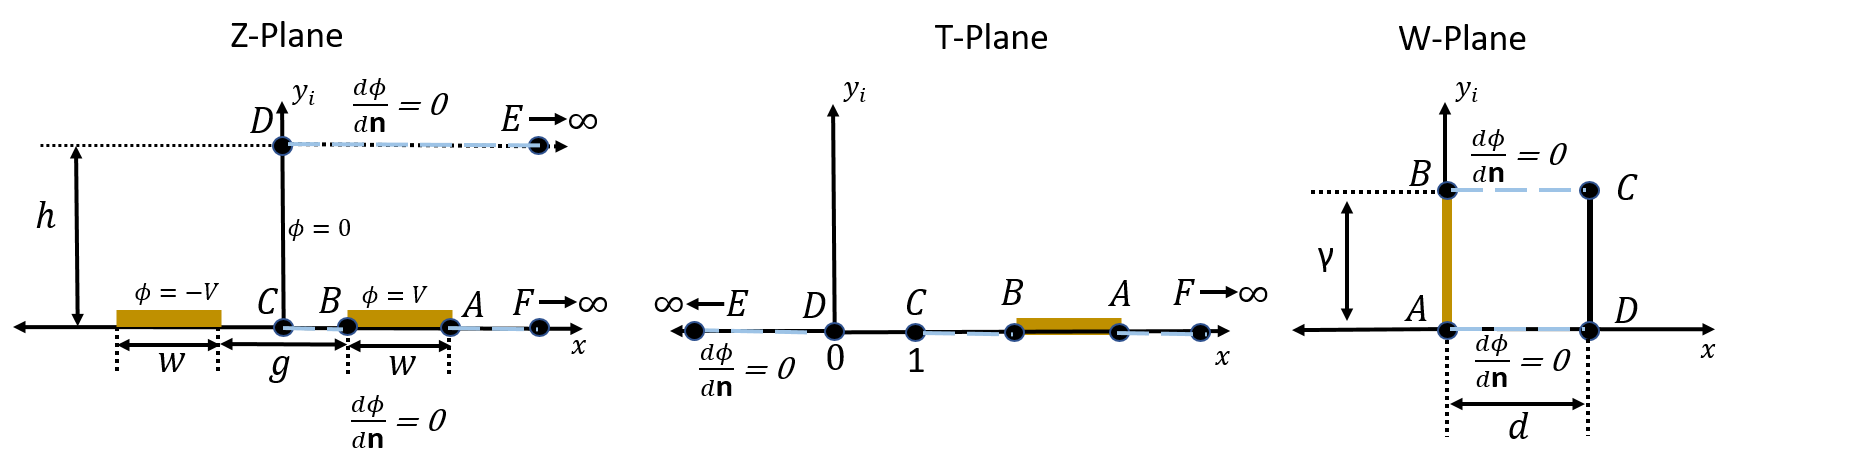
\includegraphics[width=\textwidth]{images/scmPlanes.png}
        \caption[Diagrams of coplanar electrodes through Schwartz-Christoffel mapping]{Diagrams of coplanar electrodes through Schwartz-Christoffel mapping where the Z-plane contains the physical dimensions of the electrode configuration, the T-Plane links the Schwartz-Christoffel mappins of Z and W plane, and the W-plane represents the parallel electrodes producing a uniform electrode field.}
        \label{fig:scm_planes}
    \end{figure}

\subsection*{Schwartz-Christoffel Transform Mapping}

  \par Mapping the T-plane to the Z-plane, point $C$ and $D$ will be chosen as the polygon corners with angles of $\pi/2$.  
   \begin{equation}
      Z = C_1\int (T-T_c)^{-1/2}(T-T_D)^{-1/2}dT + C_2
      \label{eqn:SCM_ZT_int}
  \end{equation}
  
 \noindent By integrating equation \ref{eqn:SCM_ZT_int} with the coordinate relationships $Z_C = 0$; $T_C = 1$ and $Z_D = jh$; $T_D = 1$, the mapping between the Z-plane and the T-plane can be expressed as
  
   \begin{equation}
     Z = \frac{2h}{\pi}\ln\Big(\sqrt{T-1} + \sqrt{T}\Big)
     \label{eqn:TZ}
 \end{equation}
 
 \noindent The mapping of the T-plane to the Z-plane is depicted in figure \ref{fig:T_to_Z_mapping}. 
 
    \begin{figure}[h]
    \centering
    \begin{subfigure}[t]{0.45\textwidth}
        \centering
        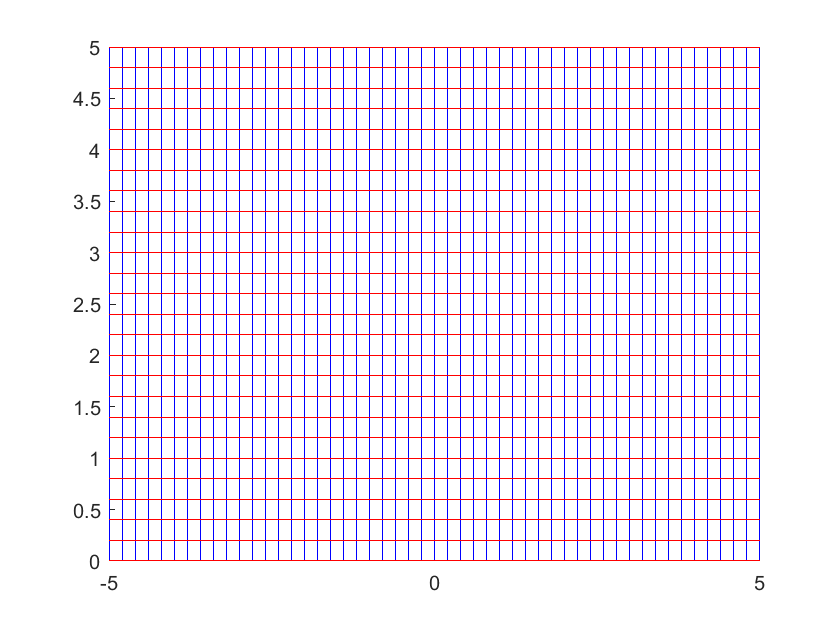
\includegraphics[width=\textwidth]{images/TtoZ_strip.png}
        \caption{Part of upper complex T-Plane}
    \end{subfigure}
    \hfill
    \begin{subfigure}[t]{0.45\textwidth}
        \centering
        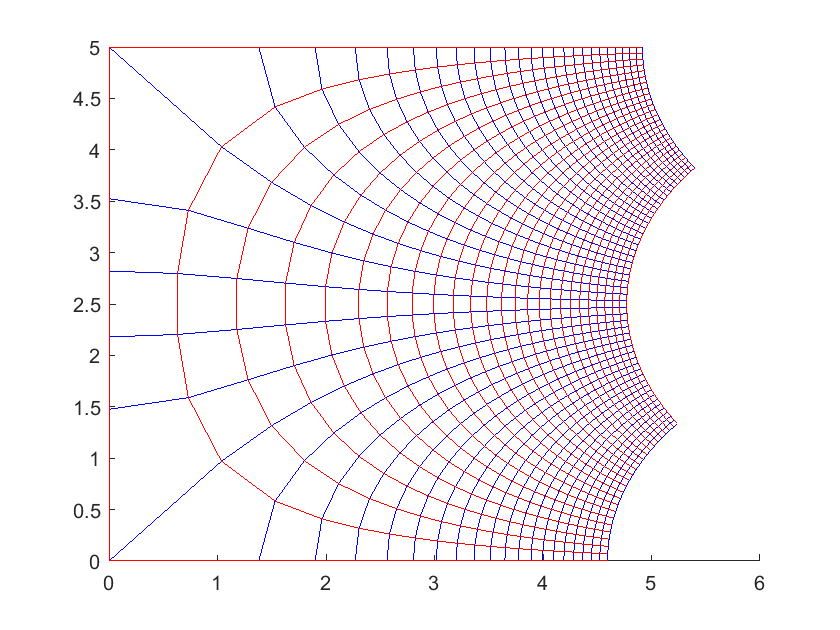
\includegraphics[width=\textwidth]{images/TtoZ_map.png}
        \caption{Mapping of the part of the T-plane to the polygon in the Z-plane}
    \end{subfigure} 
    \caption[Mapping of the T-plane to the inside of the open polygon in the Z-Plane]{Mapping of the T-plane to the inside of the open polygon in the Z-Plane outlined by the points $F$, $C$, $D$, and $E$ in the Z-plane. Equation \ref{eqn:TZ} is the mapping function.} 
    \label{fig:T_to_Z_mapping}
 \end{figure}

\par The mapping of the Z-plane to the T-plane can be found by solving for the inverse of equation \ref{eqn:TZ}.

\begin{equation}
     T = \cosh^2\bigg(\frac{z\pi}{2h}\bigg)
     \label{eqn:ZT}
 \end{equation}

\noindent Figure \ref{fig:Z_to_T_mapping} depicts the mapping of the Z-plane to the T-plane.

     \begin{figure}[h]
    \centering
    \begin{subfigure}[t]{0.45\textwidth}
        \centering
        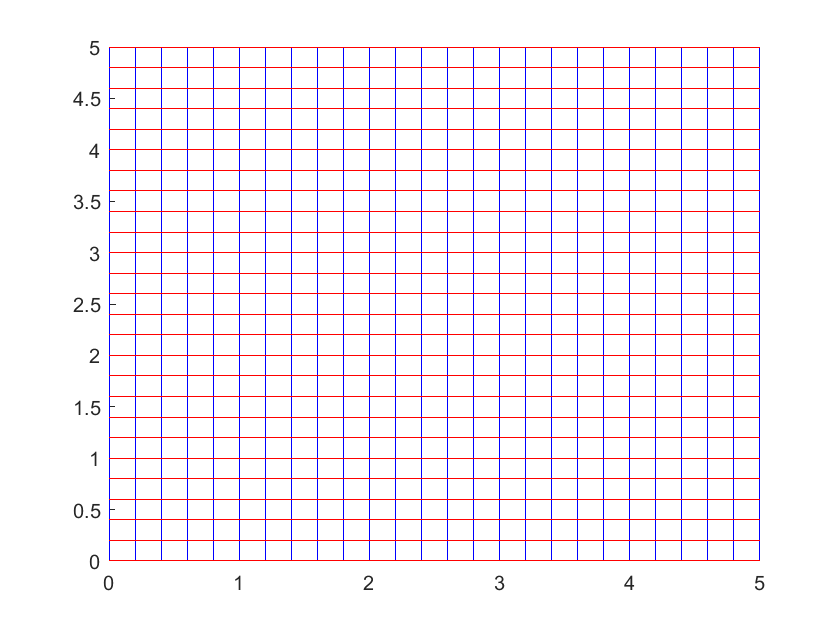
\includegraphics[width=\textwidth]{images/ZtoT_strip.png}
        \caption{Part of the open polygon in the Z-plane.}
    \end{subfigure}
    \hfill
    \begin{subfigure}[t]{0.45\textwidth}
        \centering
        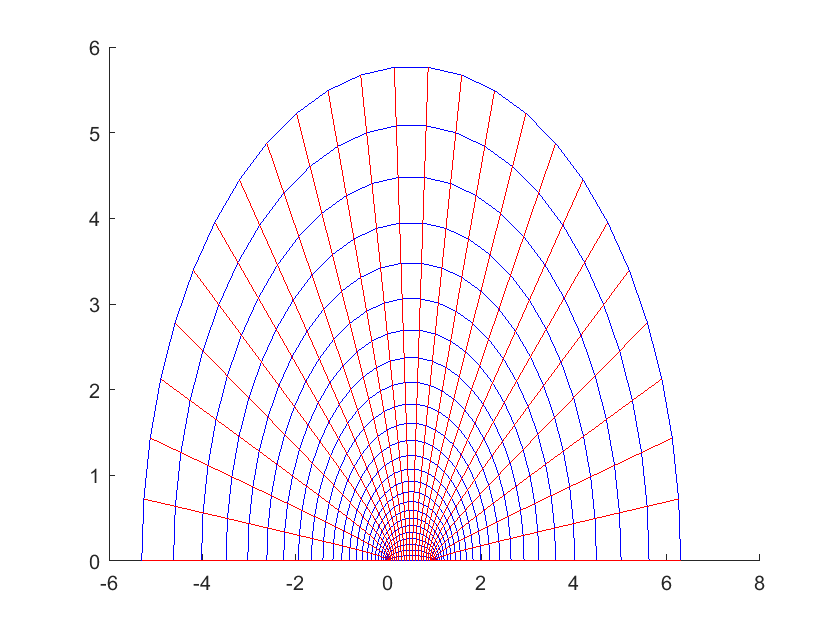
\includegraphics[width=\textwidth]{images/ZtoT_map.png}
        \caption{Mapping of part of the polygon in the Z-plane to the T-plane.}
    \end{subfigure} 
    \caption[Mapping of the open polygon in the Z-Plane to the T-plane.]{Mapping of the open polygon in the Z-Plane outlined by the points $F$, $C$, $D$, and $E$ to the T-plane. Equation \ref{eqn:ZT} is the mapping function.} 
    \label{fig:Z_to_T_mapping}
 \end{figure}

 \par Mapping the T-plane to the W-Plane, points $A$, $B$, $C$, and $D$, will be chosen as the polygon corners with angles of $\pi/2$.
 \begin{equation}
    W = D_1 \int (T-T_A)^{-1/2}(T-T_B)^{-1/2}(T-T_C)^{-1/2}(T-T_D)^{-1/2}\;dT + D_2
    \label{eqn:scm_wt_int}
 \end{equation}
 
 \noindent Since equation \ref{eqn:scm_wt_int} is an integral of a rational function with a root of a quartic polynomial, the function can be rewritten as an elliptic integral \cite{i.s._gradshteyn_table_1980}.
 
 \begin{equation}
     W = D_3F(v,k) + D_2
 \end{equation}
 \begin{equation}
    D_3 = \frac{2D_1}{\sqrt{(T_A - T_C)(T_B-T_D)}}
 \end{equation}
 
 \begin{equation}
     v = \arcsin\sqrt{\frac{(T_B-T_D)(T-T_A)}{(T_A-T_D)(T-T_B)}}
 \end{equation}
 
 \begin{equation}
     k = \sqrt{\frac{(T_B-T_C)(T_A-T_D)}{(T_A-T_C)(T_B-T_D)}}
 \end{equation}
 \noindent Where $F(v,k)$ is the incomplete elliptic integral of the first kind, and can be expressed as
 \begin{equation}
     F(v,k) = \int^v_0 \frac{d\alpha}{\sqrt{1 - k^2\sin^2\alpha}}
 \end{equation}
 \noindent Where $v$ and $k$ are referred to as the amplitude and modulus respectively.
 
 \par Using the coordinate relations for point A: $W_A = 0$, $v = 0$; point B: $W_B = j\gamma, \lim_{T\to-T_B}v = \arcsin(j\infty)$; and point D: $W_D = d$, $v = \pi/2$; we find that 
 
 \begin{equation}
     D_2 = 0
 \end{equation}
 \begin{equation}
     D_3 = \frac{d}{K(k)}
     \label{eqn:D3 w/ d}
 \end{equation}
\noindent and
\begin{equation}
    D_3 = \frac{j\gamma}{K(k')}
    \label{eqn:D3 w/ gamma}
\end{equation}

\noindent Where $K(k)$ is the complete elliptic integral and is expressed as 

 \begin{equation}
     K(k) = \int_0^{\pi/2} \frac{d\alpha}{1 - k^2\sin^2(\alpha)}
 \end{equation}
 
 \noindent and where $k'$ is the complement modulus and is expressed as 
 \begin{equation}
     k' = \sqrt{1-k^2}
 \end{equation}

\noindent By combining equations \ref{eqn:D3 w/ d} and \ref{eqn:D3 w/ gamma} we get

\begin{equation}
    \frac{\gamma}{d} = \frac{K(k')}{K(k)}
    \label{eqn:d gamma relationship}
\end{equation}

\noindent and then substituting equation \ref{eqn:d gamma relationship} into equation \ref{} we find that the cell constant for coplanar electrodes is 

\begin{equation}
    \kappa = \frac{2 K(k')}{K(k)}
\end{equation}

\par It should be noted that the current mapping T-plane to W-plane mapping is unconstrained and there is currently no solution to the constant $D_3$ without specifying a value for $d$ or $\gamma$. Physically, this is explained since the cell constant is defined by the ratio of $d$ and $gamma$. There are an infinite number of correct W-plane electrode configurations that all satisfy the ratio in equation \ref{eqn:d gamma relationship}. The relationship between all these configurations is that they all have the same impedance value. For mapping the T-plane to the W-plane, $D_3$ can be arbitrarily chosen. If $D_3$ is chosen to be 1, the T-W transform can be expressed as 

\begin{equation}
    W = F(v,k).
\end{equation}

\noindent Figure \ref{} depicts the mapping the T-plane to the W-plane. 

\subsection{Coplanar Electric Field}

 \par Now with Z-T and T-W mappings, the solution of the electric field in the W-plane can be mapped to the Z-plane. The mapping of the electric field can be expressed as 
 
 \begin{equation}
     \boldsymbol{E_z} = -\nabla \phi_z \;\;\text{with} \;\;\;\nabla \phi_z = \nabla \phi_w \overline{\frac{dW}{dZ}}
     \label{eqn:ZtoW_efield}
 \end{equation}
 
 \noindent Where $\nabla \phi$ is the gradient of potential and $\overline{\frac{dW}{dZ}}$ is the conjugate of the derivative of $W$ with respect to $Z$ \cite{schinzinger_conformal_2012}.
 
 \par Applying the chain rule to equation \ref{eqn:ZtoW_efield}, the electric field mapping is expressed as
 
 \begin{equation}
    \boldsymbol{E_z} =- \nabla \phi_w \overline{\frac{dW}{dT}\frac{dT}{dZ}}
    \label{eqn:ZtoW_efield_chain}
 \end{equation}
 
\noindent with 

 \begin{equation}
     -\nabla \phi_w = \frac{V}{d},
     \label{eqn:phi_w}
 \end{equation}
 \begin{equation}
     \frac{dW}{dT} = \frac{d}{K(k)}\frac{(T_A - T_C)^{1/2}(T_B-T_D)^{1/2}}{(T-T_A)^{1/2}(T-T_B)^{1/2}(T-T_C)^{1/2}(T-T_D)^{1/2}},
     \label{eqn:dwdt}
 \end{equation}
 \noindent and
 \begin{equation}
     \frac{dT}{dZ} = \frac{\pi}{h}(\sqrt{T-T_D})(\sqrt{T-T_C}).
     \label{eqn:dtdz}
 \end{equation}
 
 \par Combining equations, \ref{eqn:ZtoW_efield_chain}, \ref{eqn:phi_w}, \ref{eqn:dwdt}, and \ref{eqn:dtdz}, the electric field for the coplanar electrodes can be expressed as equation \ref{eqn:Ez} and is depicted with streamlines in figure \ref{fig:Ez} and as power density in figure \ref{}. A complete step-by-step solution is provided in appendix \ref{}.
 
 \begin{equation}
    E_z = \overline{\frac{\pi V}{2hK(k)} \frac{\sqrt{(T_A-T_C)(T_B-T_D)}}{\sqrt{(T-T_A)(T-T_B)}}}
    \label{eqn:Ez}
 \end{equation}
 
 
     \begin{figure}[h]
        \centering
        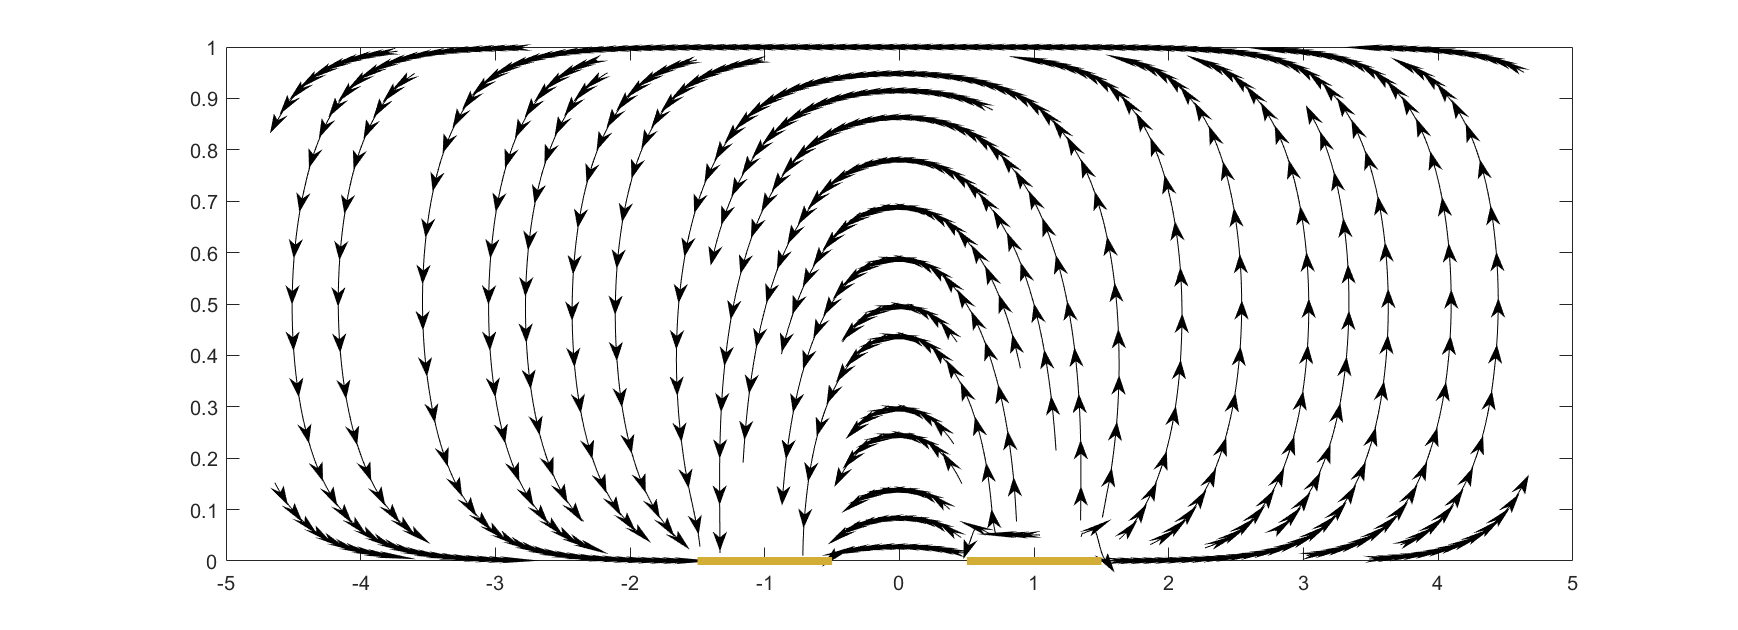
\includegraphics[width=\textwidth]{images/Ez.png}
        \caption[Electric Field for Coplanar Electrodes]{The electric field for coplanar electrodes as defined by equation \ref{eqn:Ez}.}
        \label{fig:Ez}
    \end{figure}

\subsection{Novel Volume Fraction}
\par The traditional method to approximate the volume fraction of a single particle suspended over coplanar electrodes is to take the ratio of the cell volume divided by the volume of the electrodes in the channel.

\begin{equation}
    \phi_{VR} = \frac{\frac{4}{3}\pi R^3}{(2w+g)hl}
\end{equation}

\noindent where $R$ is the particle radius, $w$ is the electrode width, $d$ is the gap between the coplanar electrodes, $h$ is the height of the channel, and $l$ is the length of the electrodes in the channel. This approximation assumes that the fringe fields outside the boundaries of the electrodes is negligible and that the electric field magnitude is uniform inside the boundaries of the electrodes. As depicted in figure \ref{}, this is not the case for coplanar electrode systems and is the reason for deriving the cell constant via conformal mapping in the first place. In this section, I propose two alternative approaches to calculating the correct volume fraction. 

\subsection*{Mapping Particle Volume to the W-Plane}
\par The shortcomings of this methods include the assumption that the mapped cross-section of the particle is an ellipse. It is not. However, as depicted in the results and discussed in the discussion, for most configurations, a spherical particle will be transformed into an ellipsoid-like particle. 

\begin{equation}
    \phi = \frac{V_{effective\;particle}}{V_{effective\;chamber}}
\end{equation}

\par One method to find the effective volumes is to calculate all volumes in the W-plane where the electric field is uniform

\begin{equation}
    V_{effective} = \int_{z}\int_{y_w}\int_{x_w} dV_w
\end{equation}

\noindent If we use the mapping to the W-plane with a constant $D_3 = 1$, the effective volume of the chamber can easily be expressed as

\begin{equation}
    V_{effective chamber} = 2K(k)K(k')l.
\end{equation}

\noindent Finding the effective volume of a spherical particle in the W-plane is harder, but can be expressed as
\begin{equation}
    
\end{equation}


\par The effective volume of the particle was approximated by assuming the spherical particle was mapped to the W-plane as an ellipsoid. 

\begin{equation}
    V_{effective} = \frac{4}{3}\pi r_{w1}r_{w2}r_{sphere}
\end{equation}

\noindent The product of the principal axis $r_{w1}$ and $r_{w2}$ were solved for by calculating the area of the orthodrome parallel to the W-plane.

\begin{equation}
    r_{w1}r_{w2} = \frac{1}{\pi}\int\int_{A_w} dA
\end{equation}

\par The volume fraction can be expressed as

\begin{equation}
    \phi_w = \frac{2}{3} \frac{r_{sphere}}{K(k)K(k')l} \int\int_{A_w} dA
\end{equation}

\subsection*{Power Volume Fraction}
\par The second approach calculates the volume fraction (or the more aptly named power fraction) as a ratio of power in the particle region to the power of the system. Intuitively, this can be rationalized by . Alternatively, it can be recalled that by its very nature, the power density in the W-plane is uniform. Furthermore, both the actual geometry and the mapped geometry contain the same amount of power. It can therefore be reasonably concluded that ratio of the power dissipated by the cell to the total power of the system is the volume fraction.

\begin{equation}
    \phi_{power} = \frac{P_{region}}{P_{system}}
\end{equation}

\begin{equation}
    P_{cell} = \int\int\int_V \rho |\boldsymbol{J}|^2 dV
\end{equation}
\begin{equation}
    P_{cell} = \int\int\int_V \rho |\frac{\boldsymbol{E}}{\rho}|^2 dV
\end{equation}
\begin{equation}
    P_{cell} = \int\int\int_V \frac{1}{\rho} |\boldsymbol{E}|^2 dV
\end{equation}
\begin{equation}
    P_{cell} = \frac{1}{\rho}\bigg(\frac{\pi^2V^2}{4h^2K(k)^2}\bigg)\int\int\int_V |\Big(\frac{T_A-T_C}{T-T_A}\Big)\Big(\frac{T_B-T_D}{T-T_B}\Big)| dV
\end{equation}

\begin{equation}
    P_{chamber} = \frac{(2V)^2}{R}
\end{equation}
\begin{equation}
    R = \rho\kappa
\end{equation}
\begin{equation}
    P_{chamber} = \frac{V^2}{\rho\kappa}
\end{equation}
\begin{equation}
    \kappa = \frac{2K(k)}{K(k')l}
\end{equation}
\begin{equation}
    P_{chamber} = \frac{V^2K(k')l}{2\rho K(k)}
\end{equation}
\begin{equation}
    \phi_{power} = \frac{\pi^2 K(k)}{8h^2K(k)K(k')l} \int\int\int_V \Bigg|\Big(\frac{T_A-T_C}{T-T_A}\Big)\Big(\frac{T_B-T_D}{T-T_B}\Big)\Bigg| dV
\end{equation}

\begin{equation}
    \phi_{power} = 2C\int^\frac{\pi}{2}_0\int^{2\pi}_0\int^R_0 r^2 \sin(\phi) f(r,\theta,\phi) drd\theta d\phi
\end{equation}

where $f(r,\theta,\phi)$ is
\begin{equation}
    f(r,\theta,\phi) = \bigg|\Big(\frac{T_A-T_C}{T(r,\theta,\phi)-T_A}\Big)\Big(\frac{T_B-T_D}{T(r,\theta,\phi)-T_B}\Big)\bigg|
\end{equation}

\begin{equation}
    Z = Z_{center} + r\cos(\pi/2-\phi)e^{i\theta}
\end{equation}

\begin{equation}
    T(r,\theta,\phi) = \cosh^2(\frac{\pi}{2h}Z_{center} + r\cos(\pi/2-\phi)e^{i\theta})
\end{equation}

%\begin{equation}
%    \phi_{power} = 2C\int^\frac{\pi}{2}_0\int^{2\pi}_0\int^R_0 r^2 \sin(\phi) \bigg|\Big(\frac{T_A-T_C}{T(r,\theta,\phi)-T_A}\Big)\Big(\frac{T_B-T_D}{T(r,\theta,\phi)-T_B}\Big)\bigg| drd\theta d\phi
%\end{equation}

\begin{equation}
    C = \frac{\pi^2}{8h^2K(k)K(k')l}
\end{equation}

\subsection*{Novel Volume fraction shortcomings}


\subsection{Device Sensitivity}
\par Linderholtz defined the sensitivity of a device as the local dissipation of power normalized by the total power of the system. In otherwords, Linderholtz sensitivity is the ratio of power density at a point in the system to the power of the system.

\begin{equation}
    S_{Linderholtz} = \frac{\rho |j|^2}{R_{sys}V_{sys}^2}
    \label{eqn:Linderholtz}
\end{equation}

\par Sun proposed an alternative sensitivity definition as the ratio or relative impedance to the impedance of the medium.

\begin{equation}
    S_{Sun} = \frac{| |\Tilde{Z}_{mix}| - |\Tilde{Z}_m| |}{|\Tilde{Z}_m|}
\end{equation}

\par Sun's definition has the advantage of taking into account the geometry of the cell and the dielectric properties of the suspension. In contrast to Linderholtz sensitivity, Sun determined that there was no optimal electrode geometry but is rather the maximization of the volume fraction. However, his calculations used the standard method of determining the volume fraction, which does not account for fringe fields and non-uniform electric fields. 

\par By using the power volume fraction with Sun's definition of sensitivity, we are essentially combining Sun's method with the ability to account for cell geometry and dielectric properties with Linderholtz's definition that takes into account the non-uniform power density of the system.

\subsection{Analytic Impedance Modeling Tool}

%%%%%%%%%%%%%%%%%%%%%%%%%%%%%%%%%%%
%%%%%% FEA Impedance Model  %%%%%%%
%%%%%%%%%%%%%%%%%%%%%%%%%%%%%%%%%%%
\section{Finite Element Analysis}

%%% Section Overview
\par Finite element analysis (FEA) models were developed to characterize the single cell impedance spectrum and to investigate optimal co-planar electrode configurations with the purpose to inform future designs. To accomplish this goal, four FEA models were designed:

\begin{itemize}
    \item Simple medium: a basic model that only includes electrodes and medium inside a rectangular domain.
    \item Simple cell: a basic model inclusive of the simple medium model with the addition of a cell centered over the electrodes.
    \item Device medium: a model that replicates the designed geometry of the Cal Poly Biofluidic Lab's impedance spectroscopy device. The model only includes electrodes and the device medium.   
    \item Device cell: inclusive of the the device medium model with the addition of a cell centered over the electrodes. 
\end{itemize}

\par Figure \ref{fig:FEA_models} depicts the four models. The simple models will investigate the characteristics of an ideal co-planar electrode cell and provide model validation by comparison to the analytic impedance solution. The device models will provide insight into the impedance characteristics of the Cal Poly Biofluidics Lab's impedance spectroscopy device. 


%%% Model Development
\subsection{Model Development}
\par The simple medium, simple cell, device medium, and device cell models were created using COMSOL Multiphyisics FEA software with the electric current physics module. Model development included the specification and implementation in COMSOL of geometry, material properties, and governing physics.

\subsection*{Model Geometry}
\par Two geometries were developed for the impedance spectroscopy models: a basic rectangular electrode cell for the simple models, and an implementation of the impedance spectroscopy device for the device models. The simple geometry is depicted in figure ## and the device geometry in figure \ref{fig:??}. The dimensions of both geometries followed the values outlined in table \ref{tab:??} with the exception of the parametric analysis and otherwise noted. In addition, a dimensioned drawing for the device geometry is included in figure \ref{fig:??}.

\par In general, the simple geometry attempts to follow two of the assumptions made in the analytic impedance solution with reference to the electrode orientation given in figure \ref{fig:??}:
\begin{enumerate}
    \item The electrode fringe fields are allowed to expand infinitely in the $\hat{\boldsymbol\imath}$ direction (i.e. there is no horizontal insulation).
    \item The electric field has no component in the $\hat{\boldsymbol\jmath}$ direction (i.e. geometry must be uniform in the direction parallel to the electrodes).
\end{enumerate}

\par The simple geometry approximated assumption 1 by making the sensor chamber sufficiently long. An iterative approach determined the sufficient length of the chamber by repeatedly increasing the length of the chamber until the model impedance stabilized to a constant value. At this point, any additional fringe fields permitted by an infinitely long channel was assumed to be negligible. This approach led to an optimal model length of NEED TO REPLACE WITH NUMBER(electrodeWidth*2 + electrode gap)*3. The second assumption was met by creating uniform features in the $\hat{\boldsymbol\jmath}$ direction.

\par The device geometry focused on the sensor chamber of the impedance spectroscope device and assumed that the effects of the electrodes far from the chamber are negligible. 

\par The cell version of both geometries includes a cell centered over the electrodes with the cell center 5 microns above the electrodes. The cell was modeled as a sphere of cytoplasm with a NEED VALUE thick membrane. 

\par Additional detail in generating the geometry model is presented in appendix \ref{app: comsol_setup}.

\subsection*{Material Properties}
\par The materials used in the FEA models included the medium solution, the cell membrane, cytoplasm, and polydimethylsiloxane (PDMS). For each of these materials materials, the conductivity and relative permittivity were specified and are summarized in table \ref{tab: fea_materials}.

\subsection*{Physics}
\par The electric current COMSOL interface was to set the physical equations for the models. The governing formula is the equation of continuity:
\begin{equation}
    \boldsymbol\nabla \boldsymbol\cdot \boldsymbol J = -\frac{d\rho}{dt}
\end{equation}

where $-\frac{d\rho}{dt}$ is the rate of change of charge density and $\boldsymbol J$ is the current density expressed as
\begin{equation}
    \boldsymbol J = \sigma\boldsymbol\E + jw\boldsymbol D + \boldsymbol J_e
\end{equation}

where \boldsymbol\E is the electric field, $j$ is $\sqrt{-1}$, $w$ is the angular frequency, $\boldsymbol J_e$ is the externally generated current density, and $\boldsymbol D$ is the electric displacement field. 

\par All exterior bound, except for the electrodes, are modeled as perfect insulators with the boundary condition
\begin{equation}
    \hat{\boldsymbol n} \boldsymbol\cdot \boldsymbol J = 0
\end{equation}

\par The cell membrane was modeled with the contact impedance condition. This is an effective alternative to meshing very thin boundaries. The condition is defined by
\begin{equation}
    \hat{\boldsymbol n} \boldsymbol\cdot \boldsymbol J = \frac{\Tilde{\sigma}}{d_{m}} \Delta V
\end{equation}

where $d_m$ is the thickness of the cell membrane and $\Tilde{\sigma}$ is the complex conductivity expressed as
\begin{equation}
    \Tilde{\sigma} = \sigma + jw\epsilon 
\end{equation}

\par The contact impedance condition only allows current normal to the selected boundary and does not allow current tangentially through the boundary. The condition can be used as an effective approximation to thin and relatively non-conductive domains. In the case of the cell membrane, it is an appropriate approximation. 

\par The low and high potential electrodes were set as the ground ($v=0$) and the applied voltage ($v=v_0$).

\par The impedance of the system was calculated by dividing the input voltage of $v_0 = 1$V by the system system current. The system current was calculated by placing a boundary probe over the ground electrode that integrated the current density over the surface of the electrode. The calculation resulted in the phasor impedance of the electrode cell. 

%%% Mesh Development
\subsection{Mesh Development}
\par For all four FEA models, quadratic tetrahedral meshes were generated. On each model a mesh convergence study based on impedance was run in order to determine appropriate meshes and validate that the model converges. To improve the simulation efficiency, the mesh was only refined in a region over the electrodes as depicted in figure \ref{fig: meshes??}.

\par The results of the mesh refinement are presented in figure \ref{fig: meshes???} and the chosen mesh with statistics are described in figure \ref{fig:meshes?}.


%%% Validation
\subsection{Model Validation}
\par The FEA models were validated by comparing the analytic impedance solutions to the results of the simple medium and simple cell models. 


%%%%%%%%%%%%%%%%%%%%%%%%%%%%%%%%%%%
%%%%%%%%  Spice Models  %%%%%%%%%%%
%%%%%%%%%%%%%%%%%%%%%%%%%%%%%%%%%%%
\section{Spice}